\documentclass{article}

% Source
%	+ https://tex.stackexchange.com/a/549546/6880
%   + https://groups.google.com/forum/#!topic/fr.comp.text.tex/X6aIq-SZDFA

\usepackage{tkz-tab}
\usetikzlibrary{calc}
\usepackage{circledsteps}

\newcommand\signline[3]{
	\coordinate (M) at ($(#1)!.5!(#2)$); 
	\path
    	(M.east) +(.75,0) pic[right]{%
			code = {
				\draw[->] (0,0)--+(0:2.5);
				\draw[blue] (0,.5)node[right=3mm]{\CircledText{\small$+$}}
				            --
				            (2.5,-.5) node[left=3mm]{\CircledText{\small$-$}};
				% Root
				\path (1.25,0) node[above,blue]{#3};
		}
	};
}


\newcommand\signparabola[4]{
	\coordinate (M) at ($(#1)!.5!(#2)$); 
	\path
    	(M.east) +(.75,0) pic[right]{%
			code = {
				\draw[->] (0,0)--+(0:2.5);
				\draw[blue] (0.25,-.6) parabola bend (1.25,.6) (2.25,-.6);
				\path (1.25,0) node[above,blue]{\CircledText{$+$}};
				\path (.275,-.3) node[left,blue]{\CircledText{$-$}};
				\path (2.25,-.3) node[right,blue]{\CircledText{$-$}};
				% Roots
				\path (.25,0) node[above,blue]{#3};
				\path (2.125,0) node[above,blue]{#4};
		}
	};
}


\newcommand\comment[3]{
	\coordinate (M) at ($(#1)!.5!(#2)$); 
	\path
    	(M.east) +(.75,0) node[right,blue]{#3}
	;
}


\begin{document}

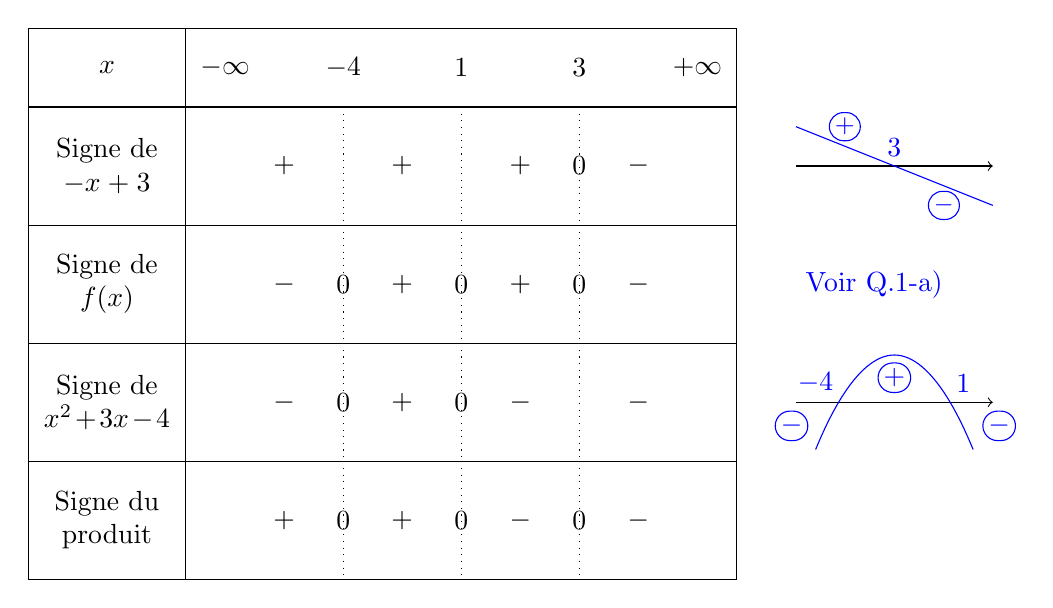
\begin{tikzpicture}
    \tkzTabInit[
    	espcl = 1.5,
%    	help % This shows TikZ names of nodes given by tkz-tab.
	]{
        $x$                         /1,
        Signe de\\ $-x+3$           /1.5,
        Signe de\\ $f(x)$           /1.5,
        Signe de\\ $x^2 + 3x - 4$   /1.5,
        Signe du\\ produit          /1.5
    }{%
         $-\infty$,    $-4$,    $1$,    $3$,   $+\infty$
    }

    \tkzTabLine { , + , t  , + , t , + , z , - }
    \tkzTabLine { , - , z  , + , z , + , z , - }
    \tkzTabLine { , - , z  , + , z , - , t , - }

    \tkzTabLine { , + , z  , + , z , - , z , - }
    
    \signline{T21}{T22}{$3$}
    \comment{T22}{T23}{Voir Q.1-a)}
    \signparabola{T23}{T24}{$-4$}{$1$}
\end{tikzpicture}

%
%\begin{tikzpicture}
%    \tkzTabInit[
%    	espcl=1.5,
%    	help% This shows TikZ names given by tkz-tab
%	]{
%        $x$                         /1,
%        Signe de\\ $-x+3$           /1.5,
%        Signe de\\ $f(x)$           /1.5,
%        Signe de\\ $x^2 + 3x - 4$   /1.5,
%        Signe du\\ produit          /1.5
%    }{%
%         $-\infty$,    $-4$,    $1$,    $3$,   $+\infty$
%    }
%
%    \tkzTabLine { , + , t  , + , t , + , z , - }
%    \tkzTabLine { , - , z  , + , z , - , z , - }
%    \tkzTabLine { , + , z  , - , z , + , t , + }
%
%    \tkzTabLine { , - , z  , - , z , - , z , + }
%\end{tikzpicture}


\end{document}